\documentclass[11pt]{article}
\usepackage[utf8]{inputenc}
\usepackage[T1]{fontenc}
\usepackage{minted}
\usepackage{graphicx}
\usepackage{hyperref}
\usepackage{CJKutf8}

\author{Student: Brian Cheung bc32427 \\ Professor: Mohit Tiwari \\ TA: Antonio Espinoza \\ Department of Electrical \& Computer Engineering \\ The University of Texas at Austin}
\date{\today}
\title{EE379K Enterprise Network Security Lab 2b Report}
\hypersetup{
 pdfauthor={Student: Brian Cheung bc32427 \\ Professor: Mohit Tiwari \\ TA: Antonio Espinoza \\ Department of Electrical \& Computer Engineering \\ The University of Texas at Austin},
 pdftitle={EE379K Enterprise Network Security Lab 2b Report},
 pdfkeywords={},
 pdfsubject={},
 pdfcreator={},
 pdflang={English}}

\begin{document}

\maketitle
\newpage
\section*{Part 3 - Orchestration}
\label{sec:part-1}
\subsection*{3a - Orchestration with Kubernetes}

\subsubsection*{Docker applications}
\noindent Questions:
\begin{enumerate}
  \item What IP address and port does the web-service use to connect to the SQL DB? Explain what you see on the homepage \verb|http://localhost:8000|.

  The port that the web-service uses to connect to the SQL DB is port 3306.
  As shown in Figure~\ref{fig:home-8000}, the web-server is serving at \verb|http://localhost:8000|.
  \begin{figure}[htbp]
    \centering
    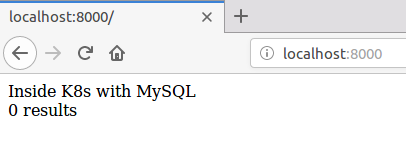
\includegraphics[width=.9\linewidth]{./home-8000.png}
    \caption{\label{fig:home-8000}
    Screenshot of the web-server serving at http://localhost:8000.}
  \end{figure}

  \item Do necessary changes so that the web-server now serves at localhost:9000. Explain the change and give screenshots.

  In order to change the port that the web-server is serving at, the host port specified in the \verb|docker-compose.yml|
  must be changed from 8000 to 9000 as shown in the code snippets below.

  The original specifications:
  \begin{minted}[highlightlines={7}]{yaml}
  ...
    website:
    container_name: php72
    build:
      context: ./
    ports:
      - 8000:80
  \end{minted}

  were changed to:
  \begin{minted}[highlightlines={7}]{yaml}
  ...
    website:
    container_name: php72
    build:
      context: ./
    ports:
      - 9000:80
  \end{minted}

  As shown in Figure~\ref{fig:home-9000}, the web-server now serves at \verb|http://localhost:9000|.
  \begin{figure}[htbp]
    \centering
    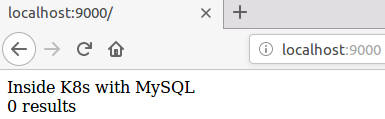
\includegraphics[width=.9\linewidth]{./home-9000.png}
    \caption{\label{fig:home-9000}
    Screenshot of the web-server serving at http://localhost:9000.}
  \end{figure}
\end{enumerate}

\subsubsection*{Kubernetes}
The first step was to tag and push the web-service image with the following commands:
\begin{minted}{bash}
  docker tag simplephpsqlk8s_website localhost:32000/simplephpsql_k8s_website:k8s
  docker push localhost:32000/simplephpsql_k8s_website
\end{minted}
To run the web-application in kubernetes:
\begin{minted}{bash}
  microk8s.kubectl apply -f webserver.yaml
  microk8s.kubectl apply -f webserver-svc.yaml
  microk8s.kubectl apply -f mysql.yaml
  microk8s.kubectl apply -f mysql-svc.yaml
\end{minted}
The following commands display information about the pods and services:
\begin{minted}{bash}
  $ microk8s.kubectl get pods --all-namespaces
  $ microk8s.kubectl get services --all-namespaces
\end{minted}
\begin{figure}[htbp]
  \centering
  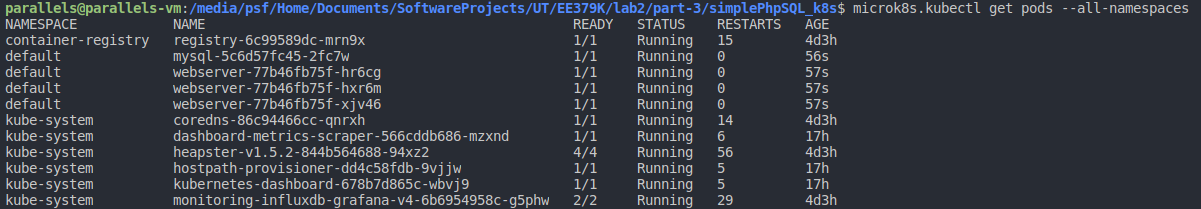
\includegraphics[width=.9\linewidth]{./pods.png}
  \caption{\label{fig:pods}
    Screenshot of the output from command microk8s.kubectl get pods --all-namespaces}
\end{figure}
\begin{figure}[htbp]
  \centering
  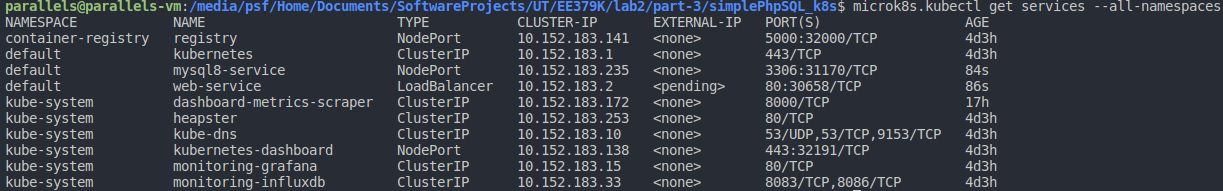
\includegraphics[width=.9\linewidth]{./services.png}
  \caption{\label{fig:services}
    Screenshot of the output from command microk8s.kubectl get services --all-namespaces}
\end{figure}

The different namespaces are specified in the NAMESPACE column in the Figures above.
\verb|kube-system| refers to the namespace created by the \verb|Kubernetes| system and includes pods/services like the dashboard.
\verb|default| is the default namespace for objects with no other namespace.~\cite{namespaces}

The number of instances of each application to be deployed is specified in the \verb|yaml| file in the \verb|replicas| field under \verb|spec|.
The original specifications of the \verb|webserver.yaml| file:
\begin{minted}[highlightlines={8}]{yaml}
  apiVersion: apps/v1
  kind: Deployment
  metadata:
    name: webserver
    labels:
      app: apache
  spec:
    replicas: 3
  ...
\end{minted}
were changed to:
\begin{minted}[highlightlines={8}]{yaml}
  apiVersion: apps/v1
  kind: Deployment
  metadata:
    name: webserver
    labels:
      app: apache
  spec:
    replicas: 2
  ...
\end{minted}
in order to deploy 2 instances of the webserver application.

The following command:
\begin{minted}{bash}
  $ microk8s.kubectl -n kube-system edit service kubernetes-dashboard
\end{minted}
opens the dashboard service script to edit the type to NodePort and find out the exposed port number of the dashboard.
The exposed port number is 32191 as specified on line 5:
\begin{minted}[linenos,highlightlines={5,12}]{yaml}
  spec:
  clusterIP: 10.152.183.138
  externalTrafficPolicy: Cluster
  ports:
  - nodePort: 32191
    port: 443
    protocol: TCP
    targetPort: 8443
  selector:
    k8s-app: kubernetes-dashboard
  sessionAffinity: None
  type: NodePort
\end{minted}

In order to open the dashboard, the secret token must be inputted to login. Once logged in,
the dashboard shows all of the pods in the default namespace as shown in Figure~\ref{fig:dashboard-def}.

In comparison to the output of running \verb|microk8s.kubectl get pods --all-namespaces| as shown in Figure~\ref{fig:pods},
not all of the pods are shown on the dashboard because the namespace of the service account is \verb|default| as specified on
line 9 of the \verb|sa-role-bind.yaml| file:
\begin{minted}[linenos,highlightlines={9}]{yaml}
kind: RoleBinding
apiVersion: rbac.authorization.k8s.io/v1
metadata:
  name: sa-rolebinding
  namespace: default
subjects:
- kind: ServiceAccount
  name: user-sa
  namespace: default
roleRef:
  kind: Role
  name: user-role
  apiGroup: rbac.authorization.k8s.io
\end{minted}
Only the pods with the default namespace are shown on the dashboard, since the service account only has access to the default namespace.~\cite{rbac}

\noindent First, create a service account named \verb|kube-system-sa| for the namespace \verb|kube-system|:
\begin{minted}{bash}
  $ microk8s.kubectl create serviceaccount kube-system-sa -n kube-system
\end{minted}

The next step is to create a role with permissions to get, list, create, update and delete.
These specificationsare defined in \verb|kube-system-role.yaml|.
Then create the role with the following command:
\begin{minted}{bash}
  $ microk8s.kubectl apply -f kube-system-role.yaml
\end{minted}

Then to bind the service account and role, a role bind yaml file must specify the service account and role.
The \verb|kube-system-sa-role-bind.yaml| file specifies to bind the \verb|kube-system-sa| service account to the \verb|kube-system-role| role.
Simply execute the following command to bind:
\begin{minted}{bash}
  $ microk8s.kubectl apply -f kube-system-sa-role-bind.yaml
\end{minted}

Next, copy the secret token to login to the dashboard.
\noindent To check if the service account was succesfully created:
\begin{minted}{bash}
  $ microk8s.kubectl get serviceaccounts -n kube-system
\end{minted}

\noindent To get the token name for the service account:
\begin{minted}{bash}
  $ microk8s.kubectl get secret -n kube-system
\end{minted}

\noindent Then get the token by specifying the token name:
\begin{minted}{bash}
  $ microk8s.kubectl describe secret kube-system-sa-token-rtv8t -n kube-system
\end{minted}

After logging in with the secret from the service account \verb|kube-system-sa|,
the dashboard displays the pods from the \verb|kube-system| namespace as shown in Figure~\ref{fig:dashboard-kube} below.
\begin{figure}[htbp]
  \centering
  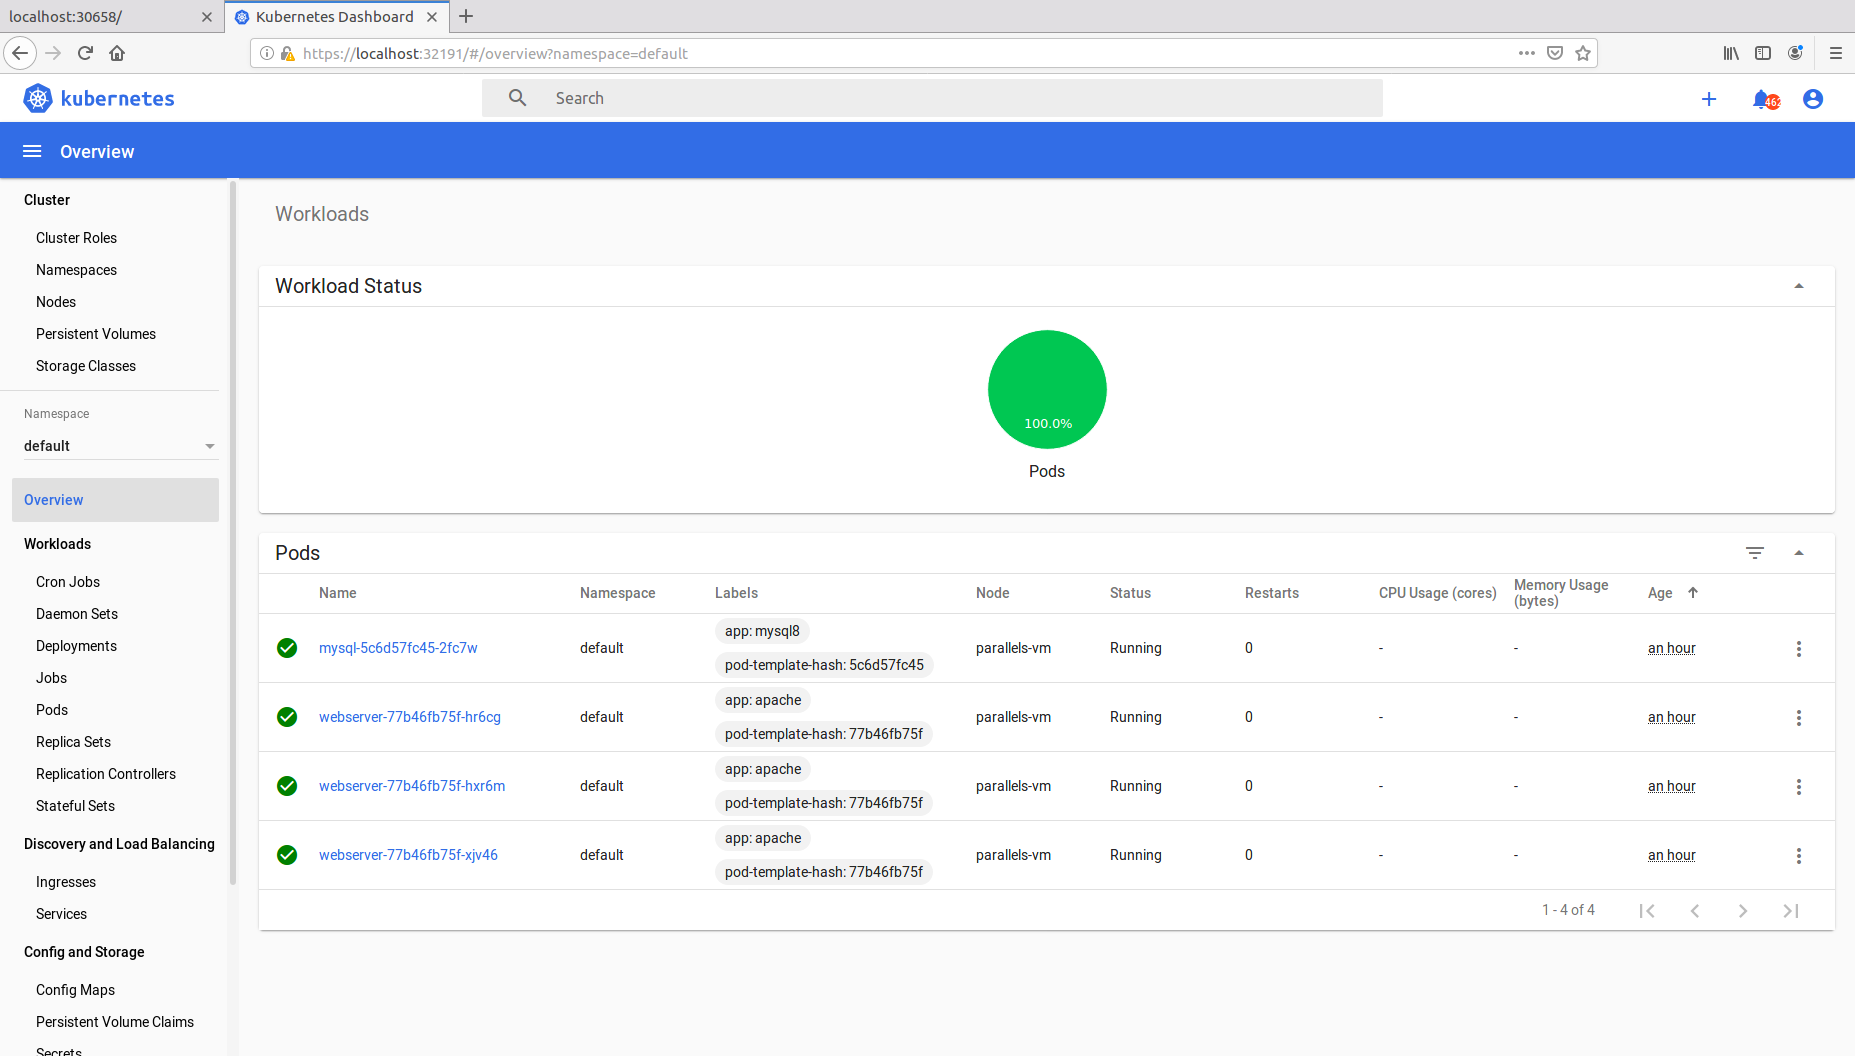
\includegraphics[width=.9\linewidth]{./dashboard-def.png}
  \caption{\label{fig:dashboard-def}
  Screenshot of the dashboard viewing the pods in the default namespace with the userS-sa service account}
\end{figure}
\begin{figure}[htbp]
  \centering
  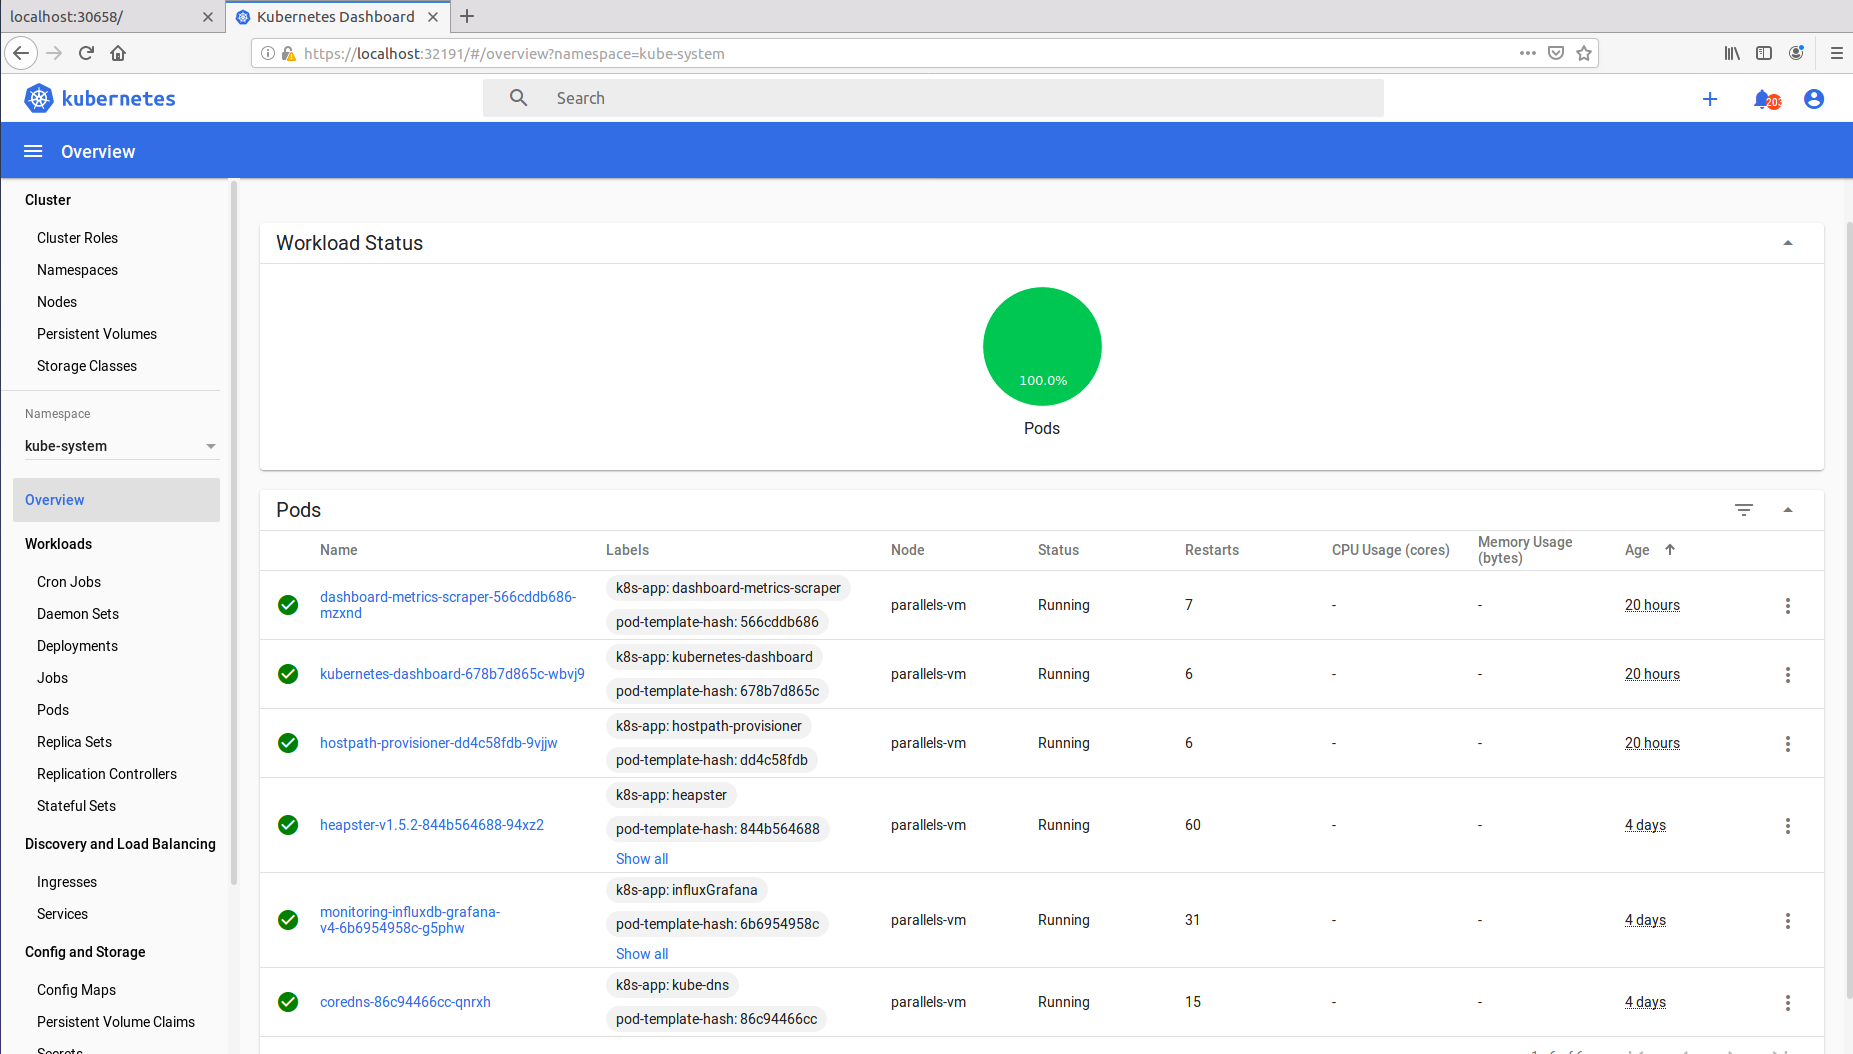
\includegraphics[width=.9\linewidth]{./dashboard-kube.png}
  \caption{\label{fig:dashboard-kube}
    Screenshot of the dashboard viewing the pods in the kube-system namespace with the kube-system-sa service account}
\end{figure}

\newpage
\subsection*{3b - Creating a kubernetes cluster for DVWA}

\section*{Conclusion}
\label{sec:conclusion}


\newpage
\nocite{*}
\bibliography{bibliography}
\bibliographystyle{ieeetr}
\end{document}
